
\documentclass[11pt]{article}
\renewcommand{\baselinestretch}{1.50}
\setlength{\textheight}{8.8in} \setlength{\textwidth}{6.3in}
\setlength{\oddsidemargin}{0.2in} \setlength{\topmargin}{-0.30in}
\setlength{\footnotesep}{10.0pt}

\usepackage{hyperref}
\hypersetup{
	colorlinks=true,
	linkcolor=black,
	filecolor=magenta,      
	urlcolor=blue,
	citecolor=black,
}



\title{{\Large \bf Industry Compliance Costs Under the Renewable Fuel Standard: Evidence from Compliance Credits\thanks{Early drafts of this paper benefited from comments by William Shughart, Ben Blau, and Megan Hansen. The Center for Growth and Opportunity at Utah State University provided financial support for data procurement and research. All errors are the author's own.}}}
\author{Arthur R. Wardle\footnote{
PhD Student, Department of Agricultural \& Resource Economics, University of California, Berkeley. \href{mailto:arw@berkeley.edu}{\tt arw@berkeley.ed} (corresponding author).}\\
Sherzod B. Akhundjanov\footnote{Assistant Professor, Department of Applied Economics, Utah State University. \href{matilto:sherzod.akhundjanov@usu.edu}{\tt sherzod.akhundjanov@usu.edu}}}

\date{May 28, 2019}

\usepackage[longnamesfirst]{natbib}
\usepackage{amsmath}
\usepackage{amsfonts}
\usepackage{tikz}
\usepackage{enumitem}
\usepackage{multirow}
\usepackage{graphicx}
\usepackage{subcaption}
\usepackage{booktabs}
\usepackage{csquotes}

\bibliographystyle{apalike}
\def\citeapos#1{\citeauthor{#1}'s (\citeyear{#1})}
\begin{document}
\maketitle

Placeholder abstract
\newline

{\small
Key Words: Biofuels, Ethanol, Refinery, Renewable Fuel Standard, Renewable Identification Numbers

JEL Classification: H23; L71; Q35; Q41; Q42; Q48}
\newpage

\section{Introduction}

The Renewable Fuel Standard (RFS), created under the Energy Policy Act of 2005 and greatly expanded by the Energy Independence and Security Act of 2007, mandates the use of various biofuels in domestic transportation fuels.\footnote{A complete description of how the RFS works is available in \cite{Schnepf2013}.} The statute itself includes volumetric mandates for cellulosic, biomass-based biodiesel, ``advanced," and total renewable fuels through 2022. Obligated parties (fuel refiners and importers) are required to submit specified numbers of Renewable Identification Numbers (RINs) to comply with the standard. RINs are created by biorefineries, which link them to barrels of renewable fuels, and are split from those barrels upon fuel blending. RINs can be traded, allowing obligated parties to comply with RFS mandates either by blending renewable fuels themselves or buying excess RINs from other parties. The construction of the RIN market is functionally equivalent to other market-based environmental regulations such as pollution permits. 

Because regulated firms can comply with the RFS either by blending additional biofuels or by buying RINs, the basic fundamental value of a RIN (with some complications, described later in this paper) is the marginal cost to the refining sector of blending an additional unit of biofuel. 

Even high RIN prices do not necessarily impact the bottom line of obligated parties if these costs are easy to pass through to consumers and demand for transportation fuels is inelastic. Indeed, a large literature establishes that refiners are able to fully (or even more than fully) pass RFS compliance costs onto consumers \citep{Burkhardt2016,Knittel2017,Pouliot2017,Li2019,Lade2019}. This, however, does not imply that the RFS has no financial impact US oil refiners whatsoever. Complete pass-through does not replace the profit margins on refined crude oil that counterfactually would  have been sold without the mandate and may impose infrastructure costs to accommodate ethanol blends, negotiating costs with biorefineries, and myriad costs of doing business not fully captured in models of cost pass-through. \cite{KnittelSmith2015} give a fuller description of ethanol's impact on oil refining profitability. The goal of our analysis is to establish how changes in the prices of RFS compliance credits (RINs) impact the value of the policy's obligated parties (refiners). To accomplish this, we implement two different reduced-form methods, which allow us to avoid imposing any particular causal channel for how the policy might impact firms' value.

\begin{figure}
	\centering
	
	\begin{tikzpicture}[node distance=1cm]
	% nodes
	\node (farm) at (0, 2) {Feedstock Farm};
	\node (rig) at (4, 2) {Oil Extraction};
	\node (biorefiner) at (0, 0) {Biorefinery};
	\node (refiner) at (4, 0) {Oil Refinery};
	\node (EPA) at (7, 0) {EPA};
	\node (blender) at (2, -2) {Fuel Blender};
	\node (retail) at (2, -4) {Gas Station};
	
	% arrows
	\draw[->]
	(farm) edge node[right] {\tiny Feedstock} (biorefiner) 
	(rig) edge node[left] {\tiny Crude} (refiner)
	(biorefiner) edge node[left] {\tiny Biofuel w/ RINs} (blender) 
	(refiner) edge node[left] {\tiny Gasoline}(blender)
	(blender) edge[bend right] node[right] {\tiny RINs} (refiner)
	(blender) edge node[right] {\tiny E10, E15, E85}(retail)
	(refiner) edge[bend right] node[below] {\tiny RINs} (EPA)
	(EPA) edge[bend right] node[above] {\tiny RVO} (refiner); 
	\end{tikzpicture}
	\caption{Obligated Parties (Oil Refiners) in a Simplified Gasoline Supply Chain}
	\label{supplychain}
\end{figure}

Outside of the academic pass-through literature, some stakeholders in RFS debates express concerns that larger refiners use the RFS to disadvantage smaller ones. Refiners in the United States can be split into ``merchant" refiners, who do not blend their own fuel and are generally smaller, and ``integrated" refiners, who do. Though refineries are the parties obligated by the RFS, RINs are not actually separated from biofuels until they are blended with gasoline. All this can be seen in Figure \ref{supplychain}, with integrated refineries owning both ``Oil Refinery" and ``Fuel Blender" assets and merchant refiners owning only the former. Not owning blending assets leaves merchant refiners in the position of having to buy RINs on the market rather than being able to generate them themselves. Merchant refiners and their advocacy organizations often claim that being unable to generate RINs puts their operations at a competitive disadvantage and allows integrated refineries to sell excess RINs for windfall profits \citep[see discussion and footnotes in][p. 21-31]{EnvironmentalProtectionAgency2017}. The Environmental Protection Agency has dismissed such arguments, pointing primarily to economic research on RIN pass-through in doing so \citep{EnvironmentalProtectionAgency2017}. Research by \cite{Babcock2016} provides a theoretical explanation for why the RFS should not impact merchant and integrated refiners differentially.

We directly examine the impact of RIN price fluctuations on the stock prices of obligated refineries. First, following \cite{Lade2018a}, who used event studies to examine how RIN price shocks affect commodity markets and biorefinery stocks, we use unanticipated regulatory announcements that drastically affected the price of RINs to identify impacts on every firm in our sample, as well as selected subgroups of firms. The two large shocks are plausibly exogenous and allow us to examine a direct response in the stock price of regulated firms. Second, we fit bivariate time series models for every possible firm $\times$ RIN combination. Modeling each firm separately allows us to investigate heterogeneity among firms. While these models provide a picture of how RINs and firm stock prices are associated over time, they are subject to endogeneity problems---both RINs and refining stocks are structurally related to commodity prices, fuel demand factors, and other variables. The intent of this paper is not to identify these structural relationships, and building them into the model is beyond the scope of this research. Instead, we use these models to cross-validate and motivate our event study models, recognizing that endogeneity issues inescapably prevent us from causally interpreting the time series results, as well as to provide a graphical idea of how shocks affect firm value using impulse response functions.

We find that when RIN prices rise, the stock prices of refineries with large market capitalizations drop with a 3-5 day lag. The effect is statistically significant though economically small. Medium and small firms, however, exhibit no reaction to RIN price changes. These results are consistent across both the event study and bivariate time series analyses. Due to the reduced-form nature of our estimates, we are unable to identify any particular causal mechanism for these results, but we conclude with a list of potential hypotheses worth investigating in future research. In any case, our findings cast doubt on claims that the RFS enables integrated refiners to take advantage of merchant refiners and suggests that the magnitude of so-called RIN ``speculation" is overblown.

\section{Background on the Renewable Fuel Standard}

The Renewable Fuel Standard is a nested mandate, meaning that blending higher-level biofuels also works to meet the mandate requirements at lower levels. RINs coming from corn ethanol generate D6 RINs, which can serve to fulfill only the lowest level of the mandate. Ethanol from more ``advanced" sources such as sugarcane generates advanced ethanol RINs (D5) and constitutes a smaller, nested mandate. RINs from biomass-based diesel (D4), cellulosic biofuel (D3), or cellulosic diesel (D7) fulfill the mandate in their own categories, the advanced mandate, and the total mandate simultaneously. This nested structure is visualized in Figure \ref{RINstructure}.

\begin{figure}[h]
	\caption{Structure of the Nested RFS Mandate}
	\label{RINstructure}
	\centering
	\begin{tikzpicture}
	\draw[rounded corners, color=black, thick] (0,0) rectangle (10,5);
	\draw[rounded corners, color=black, thick] (.2, .2) rectangle (9.8, 3.5);
	\draw[rounded corners, color=black, thick] (.4, .4) rectangle (4.9, 2);
	\draw[rounded corners, color=black, thick] (5.1, .4) rectangle (9.6, 2);
	\node[align=center] at (5,4.2) {Conventional Biofuel\\[-1ex]D6};
	\node[align=center] at (5, 2.7) {Advanced Biofuel\\[-1ex]D5};
	\node[align=center] at (2.6, 1.2) {Biomass-based Diesel\\[-1ex]D4};
	\node[align=center] at (7.3, 1.2) {Cellulosic Biofuel\\[-1ex]D3, D7};
	\end{tikzpicture}
\end{figure}
The nested relationship gives rise to a price hierarchy for RINs, which binds empirically at almost all times \citep{Whistance2014}:
$$P_{D6}\le P_{D5} \le \min \{P_{D4}, P_{D3,D7}\}$$

The absence of strictness to that inequality is not merely theoretical. Federal regulation prevents most consumer fuels (excepting E85 and E15, which contain up to 85\% and 15\$ ethanol respectively, are available at a limited number of fueling stations, and can be used only in certain vehicles) from containing more than 10\% ethanol. When national gasoline stocks are saturated with 10\% ethanol, sales of additional ethanol can occur only through comparatively miniscule E85 and E15 channels. Thus, at mandate levels beyond 10\% of nationwide gasoline sales, refiners must take advantage of the nested mandate structure and sell additional biodiesel to meet their requirements \citep{Korting2019}. In those market conditions, D6 prices track closely to D4 prices \citep{Irwin2014}.

Congress intentionally set statutory RFS volume mandates optimistically high. To prevent undue financial pressures on the transportation fuels industry, Congress explicitly allows the Environmental Protection Agency (EPA) to review the statutory volumetric standards and reduce them if compliance would be infeasible. The EPA has found it necessary to invoke that power numerous times. The following statement, released along with a proposed adjustment of the 2014-2016 mandates, illuminates the EPA's role in tempering the statutory requirements:

\begin{displayquote}
	Due to constraints in the fuel market to accommodate increasing volumes of ethanol, along with limits on the availability of non-ethanol renewable fuels, the volume targets specified by Congress in the Clean Air Act for 2014, 2015 and 2016 cannot be achieved. However, EPA recognizes that the statutory volume targets were intended to be ambitious; Congress set targets that envisioned growth at a pace that far exceeded historical growth rates. Congress clearly intended the RFS program to incentivize changes that would be unlikely to occur absent the RFS program. Thus while EPA is proposing to use the tools provided by Congress to waive the annual volumes below the statutory levels, we are proposing standards that are directionally consistent with Congress' clear goal of increasing renewable fuel production and use over time \citep{EnvironmentalProtectionAgency2015}.
\end{displayquote}

In reviewing and adjusting the yearly mandates, the EPA issues a proposed rule, gathers public comments on that proposal, and then issues a final rule. The final rule is supposed to be complete by November 30 of the preceding year (e.g., 2015's final rule should be issued by November 30, 2014). In the lifespan of the RFS, the EPA has repeatedly missed that deadline \citep{Bracmort2015}. Final rules are often made partway through the compliance year and in one case a final rule was set almost a full year after the compliance year had passed. Research by \cite{Lade2018a} demonstrates that such announcements shock RIN values as well as some commodity markets and biorefinery firm values, but no currently published research uses the shocks to identify the RFS's impact on the industry it actually regulates.

\subsection{Industry Impact}

While the RFS mandate's point of compliance generally rests with refiners, the associated costs can be pushed up or downstream if the industrial organization of markets allow it. As mentioned in the introduction, a developed literature discusses this very question. Most papers characterize the RFS as a subsidy to high-ethanol fuels and measure how changes in the value of the RIN 'subsidy' percolate to prices of E10 and E85 fuels. The general thrust of the literature concludes that pass-through is complete (or even more than complete) at the wholesale level \citep{Burkhardt2016,Knittel2017,Lade2019}, complete for E10 at the retail level \citep{Pouliot2017,Lade2019,Li2019}, and less than complete for most E85 \citep{Lade2019,Li2019}. The general interpretation of these results is that the RFS is irrelevant to the refiner, costly to most consumers, and beneficial to consumers of high-ethanol fuel and some E85 retailers.

Understanding pass-through does get us most of the way to understanding how the RFS affects refiners financially, but pass-through is not the only avenue by which the RFS could impose compliance costs. Costs associated with biofuel procurement and profit margins on gasoline sales lost to ethanol are just two additional potential ways the RFS could impose costs on refiners, even with complete pass-through. The methods undertaken in this paper impose no particular cost channel on examining the RFS's impact, instead electing to allow efficient financial markets price these anticipated costs. Examining stock price responses to variations in RIN prices gives a highly reduced-form but generalized and unstructured understanding of how the RFS impacts refineries. 

We also analyze heterogeneities among refinery responses, rather than taking refiners as a homogeneous group. Existing research on whether the impact of the RFS is heterogeneous across obligated firms is scant. There are at least a few reasons differences might exist. For example, firms which own refining capacity in close proximity to ethanol production may react less negatively to RFS cost hikes. The RIN market is designed much like pollution permits in market-based environmental policies, so that the theoretical market equilibrium in RINs should equalize the shadow prices of additional ethanol blending across firms \citep{Montgomery1972}. Whether the RIN system operates efficiently enough to effectively accomplish that is an open empirical question. Findings by \cite{LaRiviere2017} indicate that the RFS imposed heavier burdens on retail gasoline consumers distant from ethanol production centers because ethanol's physical properties make it more expensive to transport, but this is further downstream than refining and blending.

We also investigate firm size heterogeneities by asking whether larger firms have an easier time passing-through or otherwise dealing with RFS costs. Built-in exemptions for small refiners facing economic hardship seem to indicate that the drafters of the RFS policy must have worried about differential impacts. Beyond minimizing impacts on smaller refineries, exemptions can also shift the burden of meeting the volumetric mandates to larger refineries if they are issued before the final rule \citep{Coppess2017}. Exemptions hit a low point in 2015, with only 7 petitions granted representing 3 billion gallons of gasoline, as compared to 29 petitions granted representing over 13 billion gallons just two years later \citep{EnvironmentalProtectionAgency2018}. Of course, political connections, easier access to credit, and other factors benefiting large firms may mean that smaller firms still bear the brunt of the regulation. 

Large firms also tend to have integrated downstream operations, allowing them to blend their own ethanol to generate RINs rather than being required to buy them from separated downstream blenders. As discussed in the introduction, this is the basis for a perennial complaint by small refineries, who argue that integrated operations profit from their ability to generate and sell their excess RINs. 

All sorts of heterogeneities in firm operations are of interest to regulatory agencies because differences in cost structures could counter-intuitively incite lower-cost firms to support the law as a new, artificial source of comparative advantage \citep{Salop1983}. Our reduced-form estimates of how firms respond to positive price changes in RFS compliance costs can lend credence to or discredit some of these theories.

\subsection{2015 RIN Shocks} \label{sec_2015shocks}

As mentioned previously, the EPA sometimes misses regulatory announcement deadlines, resulting in major regulatory announcements that occur mid-compliance year. In 2013, the EPA released the final rule on August 6, leaked a draft proposal for 2014 on October 11, and released 2014's official proposed rule on November 15. \cite{Lade2018a} measures how 2013's mid-year announcements influenced RIN prices themselves, related commodity markets, and the stock prices of biorefining firms.  They find that those shocks, which drove the prices of all RIN varieties downward, mainly impacted commodities and firms tied to advanced biofuels, which they considered to be the marginal compliance fuel. The year 2013 was a volatile time for RIN markets, and visual inspection of RIN price histories throughout 2013 in Figure \ref{2013pricehistory} reveals that the announcement dates analyzed by \cite{Lade2018a}, while significant, are unremarkable compared to baseline volatility.

%\begin{figure}[h]
%	\caption{Price Histories for 2013 Vintage RINs}
%	\label{2013pricehistory}
%	\includegraphics[width=\textwidth]{Figures/2013RINs.pdf}
%\end{figure} 

Unlike 2013, 2015's proposed and final rules, which were released on May 29 and November 30, are clearly and unambiguously apparent by visual inspection of Figure \ref{2015pricehistory}.\footnote{In an online supplement, \cite{Lade2018a} repeat the portion of their analysis detailing how policy announcements affect RIN prices for 2015 event dates. Unlike their 2013 analysis, they do not examine how 2015 announcements affected biofuel stocks or commodity markets.} Surrounding a proposed rulemaking on May 29, 2015, the price of a D6 RIN dropped from \$0.69 one week before to \$0.3775 one week afterwards, a drop of more than 45\%. A jump of similar magnitude surrounded a final rulemaking on November 30, 2015. 

\begin{figure}[h]
	\caption{Price History for 2015 Vintage RINs}
	\label{2015pricehistory}
	\includegraphics[width=\textwidth]{figures/2015RINs}
\end{figure}

In this study, we focus on 2015 because the EPA made two major policy announcements that we will exploit as structural breaks following \cite{Lade2018a}. We choose 2015 over 2013, the primary year analyzed by \cite{Lade2018a}, for two reasons: First, the announcement breaks are much clearer in the data; that can be seen by comparing Figures \ref{2013pricehistory} and \ref{2015pricehistory}, but note the change in the extent of the price axis. Second, RIN prices are sufficiently high throughout 2015 to guarantee that the mandate was binding, whereas early 2013 prices were so low that the RFS may not have actually been stringent enough to alter refiner behavior \citep{Whistance2016}.

\subsection{Identification of RFS Industry Impact}

This paper employs two methodologies to study the impact of the Renewable Fuel Standard on the refining industry. First, we use multivariate time series methods to quantify the response of refining firm values to shocks in RIN price series. In particular, for every Firm $\times$ RIN combination, we estimate impulse response functions using vector auto-regressions and vector error correction models. These allow us to determine the dynamic response of the value of refining firms to shocks in the value of RIN prices. This portion of our analysis builds on past literature using time series methods to unravel how RINs transmit to wholesale and consumer fuels \citep{Knittel2017} and biofuel-related commodities \citep{Whistance2014, Whistance2016}. Second, we implement an event study methodology similar to that used by \cite{Lade2018a}. Even if endogeneity complicates measurement of direct industry impact using conventional multivariate time series methods, we anticipate that the large shocks constituting nearly half of RIN prices should induce measurable impacts on refining firms if indeed there is an impact. The event study methodology also side-steps nonlinearities in the RIN-stock system that may complicate the bivariate models \citep{Serra2011}.

Both methodologies are reduced-form. By examining stock prices rather than specific product prices, we should be able to identify the impact of \textit{any} channel whereby a larger RFS mandate influences the net values of refining firms in the short-run. The downside of this approach is that we cannot validate any particular channel of causality. Nevertheless, establishing the existence or non-existence of an effect in and of itself offers insights as to whether cost pass-through is an adequate stopping point for research seeking to understand how regulated industries respond to the RFS and other fuel blend regulations.

\section{Data}

As described in the introduction, RINs are compliance credits that refiners obligated by the RFS can use to meet their biofuel utilization mandates. Because multiple, nested categories exist within the RFS mandate, there are four commonly traded types of RINs, as shown in Figure \ref{RINstructure}.

The mandate for D3 RINs is consistently minuscule, and markets for those RINs are commensurately quite thin. Therefore, we restrict our analysis to D6, D5, and D4 RINs. RIN series also differ by their year of creation; apart from some flexibility allowing limited inter-year banking and borrowing of RIN stocks, RINs are mostly used to comply with the mandate for the year in which they were generated. Thus, we limit our analysis to RINs of a single compliance year.\footnote{The majority of the literature examining RIN prices do not restrict their analyses to a single compliance year. It is not always clear how this literature stitches together price series for RINs belonging to difference compliance years, especially when RINs for multiple compliance years are sold contemporaneously.} As discussed in Section \ref{sec_2015shocks}, we analyze data from 2015. Because of some pre-year trading and the fact that RINs are not actually submitted for compliance until a few months after year end, our data does extend a little beyond a single calendar year. 

All data is daily, excluding weekend and other financial market closures such as holidays. Data for RIN series come from the Oil Price Information Service (OPIS), a company that provides pricing for numerous petroleum products and is a frequent supplier of RIN data for economic researchers. Stock prices for nearly all firms are adjusted prices from Yahoo! Finance (accessed via the quantmod package in R). Stocks delisted since 2015 are not available on Yahoo! Finance and are instead sourced from Bloomberg. While these prices are not adjusted, none of those firms underwent stock splits or reverse-splits in the study period, so this should be of little consequence.

\subsection{Firm Characteristics}\label{sec_firmcharacter}
This study encompasses all publicly traded firms with at least 200,000 barrels per day of refining capacity as of January 1, 2015, plus Western Refining \citep{EnergyInformationAdministration2015}. We sort firms along two dimensions: size and exposure to RFS regulatory costs as of the beginning of 2015. We use market capitalization as a relevant measure of firm size \citep{Fama1992} and the percentage of a firm's refining capacity in PADD 2 and Alaska as our measure of exposure (or, rather, non-exposure).\footnote{PADD stands for Petroleum Administration for Defense Districts. Using refining capacity in PADDs 2, 3, and Alaska or, inversely, using refining capacity in PADDs 1 and 5 minus Alaska, hardly changes the groupings.}

PADDs are collections of states by which many government-issued petroleum data sources are aggregated. The Midwest, encompassed by PADD 2, contains the vast majority of ethanol refining capacity because refinery location decisions are driven primarily by access to feedstocks \citep{Lambert2008}. Because ethanol cannot be transported using existing pipeline infrastructure, it is plausible to think that the RFS puts refineries located near biorefineries at a comparative advantage. Geographic disparity in the impacts of the RFS have already been documented for retail gasoline prices \citep{LaRiviere2017} and pass-through of RIN prices by rack sellers at fuel terminals \citep{Pouliot2017}. Alaskan refining capacity is also included in this measure because Alaska is exempted from the RFS. We sort firms into one of nine bins, one for each element of the cross product of three market capitalization and three RFS exposure bins, as shown in Table \ref{bins}. The cutoffs were chosen somewhat arbitrarily to result in balanced bins, but, as the next paragraph further explains, the cutoffs do run parallel to important qualitative differences between firms.

Firms characterized as large (market capitalizations in excess of \$100B) are also the US firms generally considered to be large, integrated refineries: BP, Shell, Chevron, and ExxonMobil. In mid-2015, an analysis released by Valero Energy Corporation argued that those firms were already separating RINs in excess of their own RFS obligations, yielding them ``windfall profits," because their sales of branded gasoline made up large percentages of their refinery production \citep{ValeroEnergyCorporation2016}. Patterns of price response among these energy firms could lend evidence for or against those conjectures. The line between small and medium refining firms also separates relatively smaller nationwide operations from merely regional companies. 

\begin{table}[h]
	\caption{Firm Characteristics with Ticker Symbols}
	\label{bins}
	\centering
	\resizebox{\textwidth}{!}{
		\begin{tabular}{l c c c }
			\hline
			\hline
			& 100\% Exposed		&$<$100\% \& $>$70\% Exposed 			& $<$70\% Exposed\\
			\hline
			
			Large:  &	Shell (RDS.A)		& 		&			 \\
			$>$\$100B	& Chevron (CVX)		& Exxon Mobil (XOM)						&British Petroleum (BP) \\	 
			& 	Total (TOT)			& 						& 			\\ \\
			
			Medium:& 						& Valero (VLO)			& \multirow{2}{*}{Marathon (MPC)}		\\
			$<\$$100B, $>\$$10B 	& 					& Phillips 66 (PSX)		& \\ \\
			
			Small: &Carlyle Group (CG)		&\multirow{2}{*}{Andeavor (ANDV)}						& \multirow{2}{*}{HollyFrontier (HFC)}\\
			$<$\$10B&Western Refining (WNR)	& 		& \\
			\hline			
			
		\end{tabular}
	}
\end{table}


\subsection{Stationarity Tests}

Both methods of our analysis require stationary data inputs, so we begin by testing for stationarity in our data. Tests for stationarity are known to be biased towards conclusions of non-stationarity in the presence of structural breaks \citep{Perron1989}. However, despite evidence indicating the presence of structural breaks in RIN price series \citep{Mason2016,Lade2018a}, no prior research to our knowledge considers structural breaks in tests of RIN price stationarity, including RFS research specifically related to large breaks, such as \cite{Lade2018a}. 

Most popular structural break tests allow for endogenous breakpoint selection, reflecting that most structural break research requires first identifying the exact location of the breakage. We have no need for that---we know the precise dates of the breaks ex ante---and running those tests would sacrifice power unnecessarily. \cite{Lee2003} depart from that norm and offer a stationarity test (hereafter the LS test) that allows for up to two exogenously defined structural breaks.\footnote{An endogenous version of the same test is also described by \cite{Lee2003} and is the test most frequently associated with the paper.}

The LS test allows for breaks in both mean and trend, using a vector of structural break variables for breaks occurring at $t=T_1$ and $t=T_2$:  $Z_t=[DU_{1,t},DU_{2,t},DT_{1,t},DT_{2,t}]'$, where $DU_{i,t}=1$ for $t\ge T_i+1$ and zero otherwise and $DT_{i,t}=t-T_i$ for $t\ge T_i+1$ and zero otherwise for $i=1,2$. The LS two-break unit root test is estimated by the equation
\begin{equation}
\Delta y_t=\delta'\Delta Z_t+\phi \tilde{S}_{t-1}+u_t,
\end{equation}

\noindent where $y_t$ is the variable whose stationarity is being tested; $\Delta$ is the difference operator; $\tilde{S}_t=y_t-\tilde{\psi}_x-Z_t\tilde{\delta}$ for $t\ge2$; $\tilde{\delta}$ are coefficients recovered from a regression of $\Delta y_t$ on $\Delta Z_t$ (i.e., $\Delta y_t=\delta'\Delta Z_t+e_t$);  $\tilde{\psi}_x=y_1-Z_1\tilde{\delta}$; and $u_t$ satisfies the normality conditions defined by \citet[p. 336]{Phillips1988}. The test statistic for the unit root null hypothesis is the $t$-statistic on the parameter estimate for $\phi$, and significance is checked using critical values for an exogenous 2-break unit root test reported in \cite{Lee2003}.\footnote{\cite{Lee2003} only report critical values for tests with a sample size of 100, whereas our sample size is 357. This will result in the test being underpowered.}

For testing stationarity of our non-RIN series, the LS test conveniently exhibits nice size and power properties even when the actual data generating process contains no breaks. Results of the LS test are reported in Table \ref{stationarity} alongside the typical Augmented Dickey-Fuller (ADF) and Kwiatkowski-Phillips-Schmidt-Shin (KPSS) tests, which do not account for structural breaks. The three tests conclude unanimously that every RIN and stock price series is non-stationary. 



\begin{table}[htbp] \centering 
	\caption{Summary Statistics and Stationarity Tests} 
	\label{stationarity} 
	\begin{tabular}{@{\extracolsep{5pt}} lcccccc} 
		\hline 
		\hline \\[-1.8ex] 
		& \multicolumn{3}{c}{Summary Statistics}  & \multicolumn{3}{c}{Stationarity Tests}\\
		\cmidrule(r){2-4} \cmidrule(r){5-7}
		& Mean & St. Dev & Obs.        & ADF & KPSS & LS \\ 
		\hline
		Null & 	   &       &    & Non-stationary & Stationary & Non-stationary \\
		\hline \\[-1.8ex] 
		\input{tables/stationarity_edited.tex}
		\hline
	\end{tabular} 
\begin{flushleft}
\scriptsize{Significance at alpha levels of 0.1, 0.05, and 0.01 are reported with *, **, and ***, respectively.}\\
\end{flushleft}
\end{table}  



\begin{table}[!htbp] \centering 
	\caption{Results from Event Studies} 
	\label{eventstudies} 
	\resizebox{.7\textwidth}{!}{
		\begin{tabular}{@{\extracolsep{5pt}} lcccc} 
			\hline 
			\hline \\[-1.8ex] 
			& Large Firms & Medium Firms & Small Firms & All Firms \\ 
			\hline \\[-3.6ex] 
			{\it \textbf{Event 1}} & & & & \\
			\input{tables/event_studies_edited.tex}
			\hline 
		\end{tabular} 
	}
	\begin{flushleft}
		\scriptsize{Note: Significance at alpha levels of 0.1, 0.05, and 0.01 are reported with *, **, and ***, respectively.}\\
	\end{flushleft}
\end{table} 

\begin{table}[!htbp] \centering 
	\caption{Cointegration Tests} 
	\label{cointegration} 
	\begin{tabular}{@{\extracolsep{5pt}} lcccccc} 
		\hline 
		\hline \\[-1.8ex] 
		&\multicolumn{3}{c}{Maximum Eigenvalue} & \multicolumn{3}{c}{Trace}\\
		\cmidrule(r){2-4} \cmidrule(r){5-7} \\[-1.8ex]
		Firm& D6 & D5 & D4 & D6 & D5 & D4 \\ 
		\hline \\[-1.8ex] 
		\input{tables/cointegration_edited.tex}
		\hline
	\end{tabular} 
	\begin{flushleft}
		\scriptsize{Note:  Significance at alpha levels of 0.1, 0.05, and 0.01 are reported with *, **, and ***, respectively.}\\
	\end{flushleft}
\end{table} 



\begin{table}[!htbp] \centering 
	\caption{Bivariate Time Series Model with D6 RINs} 
	\label{d6timeseries} 
	\resizebox{\textwidth}{!}{
		\begin{tabular}{@{\extracolsep{0pt}} lcccccccccccc} 
			\hline 
			\hline \\[-1.8ex] 
			\input{tables/D6VAR_edited.tex}
			\hline 
		\end{tabular} 
	}
\begin{flushleft}
\scriptsize{Note:  Significance at alpha levels of 0.1, 0.05, and 0.01 are reported with *, **, and ***, respectively.}\\
\end{flushleft}
\end{table} 

\begin{table}[!htbp] \centering 
	\caption{Bivariate Time Series Model with D5 RINs} 
	\label{d6timeseries} 
	\resizebox{\textwidth}{!}{
		\begin{tabular}{@{\extracolsep{0pt}} lcccccccccccc} 
			\hline 
			\hline \\[-1.8ex] 
			\input{tables/D5VAR_edited.tex}
			\hline 
		\end{tabular} 
	}
	\begin{flushleft}
		\scriptsize{Note:  Significance at alpha levels of 0.1, 0.05, and 0.01 are reported with *, **, and ***, respectively.}\\
	\end{flushleft}
\end{table} 

\begin{table}[!htbp] \centering 
	\caption{Bivariate Time Series Model with D4 RINs} 
	\label{d6timeseries} 
	\resizebox{\textwidth}{!}{
		\begin{tabular}{@{\extracolsep{0pt}} lcccccccccccc} 
			\hline 
			\hline \\[-1.8ex] 
			\input{tables/D4VAR_edited.tex}
			\hline 
		\end{tabular} 
	}
	\begin{flushleft}
		\scriptsize{Note:  Significance at alpha levels of 0.1, 0.05, and 0.01 are reported with *, **, and ***, respectively.}\\
	\end{flushleft}
\end{table} 
\section{Conclusion}

Just a test conclusion

\newpage



\bibliography{references}


\end{document}